\chapter{Object reconstruction}
\chaptermark{Object reconstruction}  
\thispagestyle{plain}  % First page has default style
\pagestyle{chapterpages}
\label{Section:Chapter4}
\minitoc

This chapter presents the reconstruction of physics objects in the CMS detector, which is foundational to all analyses performed in this thesis. In particular, $\PGt$ lepton reconstruction is a central focus. The reconstruction of $\PGt$ leptons is particularly challenging due to their short lifetime and complex decay modes, which can involve a mix of charged and neutral hadrons, electrons, muons, and undetectable neutrinos. Therefore, accurate $\PGt$ identification requires the excellent performance of multiple reconstruction components, including \textit{charged-particle tracking}, \textit{electromagnetic} and \textit{hadronic calorimetry}, \textit{muon identification}, and \textit{displaced secondary vertexing}.

However, operating in a high-multiplicity environment introduces additional challenges for the reconstruction and identification of physics objects. There is no guarantee that a reconstructed particle corresponds to a genuine physics object; such cases are referred to as \textit{misidentified} or \textit{``fake'' objects}. For example, jets initiated by quarks or gluons can sometimes be misidentified as hadronic $\PGt$ decays; leptons originating from heavy-flavour decays within jets may mimic prompt electrons or muons; and, conversely, muons and electrons can occasionally be misidentified as jets. To mitigate these effects, object identification algorithms incorporate \textit{multivariate discriminants} and \textit{\acp{WP}} that are tuned to balance efficiency and misidentification rates. However, in some cases, these strategies only partially suppress such backgrounds.

A more complete and accurate event description is achieved by correlating information from all layers of the CMS detector to reconstruct and identify individual particles. This integrated methodology is known as \ac{PF} reconstruction. The implementation of this approach within CMS is detailed in this chapter.

\section{Reconstruction of Particle Flow detector elements}
\label{Section:Chapter4_Reconstruction_of_PF_elements}
\subsection{Track reconstruction}

The first stage of the reconstruction process, known as \textbf{local reconstruction}~\cite{CMS_TrackerPerformance_2014,CMS_Track_Reconstruction_Run2_3}, involves clustering zero-suppressed signals above predefined thresholds in the tracker sensors to form hits, referred to as \textit{clusters}. For each cluster, both the position and its associated uncertainty are estimated within a local coordinate system defined by the sensor geometry. These locally reconstructed hits form the basis for the subsequent \textbf{global reconstruction}~\cite{CMS_TrackerPerformance_2014,CMS_Track_Reconstruction_Run2_3} of particle trajectories.

Global track reconstruction at CMS is facilitated by the \textbf{\ac{CTF}} algorithm~\cite{CMS_TrackerPerformance_2014,CMS_Track_Reconstruction_Run2_3}, an adaptation of the combinatorial \textit{\ac{KF}}~\cite{KF_1,KF_2,KF_3}\footnote{KF~\cite{KF_4} is recursive algorithm that uses a series of measurements over time to estimate the state of a system. This is done by estimating a joint probability distribution over the variables of interest at each time step.} approach. This adaptation enables pattern recognition and track fitting to be performed within a unified framework, allowing hits to be incrementally added and track parameters to be continuously updated in a process known as \textbf{iterative tracking}. A single iteration of the CTF algorithm proceeds in four steps:

\begin{enumerate}
    \item \textbf{Seed generation}: Initial track candidates are formed using a small number of hits (typically two or three) in the innermost layers of the tracker. Each \textit{seed} provides an initial estimate of the particle's trajectory parameters, such as position, direction, and momentum, as well as their associated uncertainties. 
    \item \textbf{Track finding}: Seed trajectories are extrapolated along the expected trajectory of a charged particle using a Kalman Filter (KF). At each detector layer, additional hits along the expected flight path are identified and associated with the track candidate; the trajectory parameters are then updated accordingly. This process is repeated iteratively until the outermost layer of the detector is reached, gradually building complete track candidates from the initial seeds.
    \item \textbf{Track fitting}: The final trajectory is refitted iteratively to improve the estimate of the track parameters. This is done using a combination of a KF and a smoother, incorporating all available hit information.
    \item \textbf{Track selection}: Tracks are required to pass a set of quality flags.
\end{enumerate}

The \textbf{iterative tracking} procedure in CMS is performed in successive iterations, each designed to target different classes of tracks, as summarised in Table~\ref{Table:Chapter4_IterativeTrackingSeeds}. The initial iterations target tracks that are the easiest to find (\eg high $p_\mathrm{T}$ tracks, and tracks produced near the primary interaction point). After each iteration, the combinatorial complexity is reduced by removing hits associated with tracks. This enables later iterations to target more challenging classes of tracks (\eg low $p_\mathrm{T}$ tracks, and tracks displaced from the interaction point). 

\begin{table}[h]
\centering
\renewcommand{\arraystretch}{1.5} % Increase row height
\arrayrulecolor{black} % Ensure outer borders are black
\begin{tabular}{|c|l|l|l|}
\hline
Iteration & Name & Seeding & Targeted Tracks \\ \hline \hline
1         & InitialStep              & pixel triplets              & prompt, high $p_\mathrm{T}$                     \\
\arrayrulecolor{lightgray} \hline
2         & DetachedTriplet          & pixel triplets              & b hadron decays, R $\leq 5\unit{cm}$      \\
\arrayrulecolor{lightgray} \hline
3         & LowPtTriplet             & pixel triplets              & prompt, low $p_\mathrm{T}$                      \\
\arrayrulecolor{lightgray} \hline
4         & PixelPair                & pixel pairs                 & recover high $p_\mathrm{T}$                     \\
\arrayrulecolor{lightgray} \hline
5         & MixedTriplet             & pixel+strip triplets        & displaced, R $\leq 7\unit{cm}$                \\
\arrayrulecolor{lightgray} \hline
6         & PixelLess                & strip triplets/pairs        & very displaced, R $\leq 25\unit{cm}$          \\
\arrayrulecolor{lightgray} \hline
7         & TobTec                   & strip triplets/pairs        & very displaced, R $\leq 60\unit{cm}$          \\
\arrayrulecolor{lightgray} \hline
8         & JetCoreRegional          & pixel+strip pairs           & inside high $p_\mathrm{T}$ jets                 \\
\arrayrulecolor{lightgray} \hline
9         & MuonSeededInOut          & muon-tagged tracks          & muons                               \\
\arrayrulecolor{lightgray} \hline
10        & MuonSeededOutIn          & muon detectors              & muons                               \\
\arrayrulecolor{black} \hline
\end{tabular}
\caption[Summary of iterative tracking steps in CMS]{Summary of the iterations used in the CMS iterative tracking algorithm. Table taken from Ref.~\cite{ParticleFlow}.}
\label{Table:Chapter4_IterativeTrackingSeeds}
\end{table}

\subsection{Vertex reconstruction}

The primary goal of the CMS vertex reconstruction~\cite{CMS_TrackerPerformance_2014} is to determine the positions and associated uncertainties of all proton-proton interaction vertices in an event, including both the \textbf{\ac{PV}} (associated with the \textit{``signal'' interaction}) and any additional vertices originating from PU collisions, using all available reconstructed tracks. The reconstruction process is performed in three main steps: 

\begin{enumerate}
    \item \textbf{Track selection}: Tracks consistent with originating promptly near the centre of the luminous region (referred to as the beam spot) are selected. This selection is based on applying quality requirements to the tracks, such as cuts on the transverse impact parameter significance relative to the beam spot and minimum numbers of associated pixel and strip hits.
    \item \textbf{Track clustering}: Tracks are clustered into groups that appear to be originating from the same vertex. This clustering is performed based on their z-coordinate at the point of closest approach to the beam spot using a \textit{deterministic annealing algorithm}~\cite{DeterministicAnnealing}.
    \item \textbf{Vertex fitting}: Candidate vertices composed of at least two tracks are fitted using an \textit{adaptive vertex fitter}~\cite{VertexFitting_2006,VertexFitting_2007} to determine the best estimate of the vertex parameters. These parameters include the $x$, $y$, and $z$ positions, the associated covariance matrix, and indicators of fit quality. Additionally, the adaptive fit assigns a weight between 0 and 1 to each track, reflecting the probability that the track is genuinely associated with the vertex.
\end{enumerate}

Once all the vertices are reconstructed, a collection is formed, which is ordered by the quadratic sum of the transverse track momenta associated with each vertex, $\sum_{\text{tracks}} p_{\mathrm{T}}^2$. The vertex with the largest sum is assumed to most likely correspond to the vertex of the hard scattering process~\cite{ParticleFlow}. The efficiency to correctly identify the PV when at least three tracks are associated is close to 100\%~\cite{CMS_TrackerPerformance_2014}. The resolution of the PV position, particularly in the $x$ and $z$ coordinates, has been measured using $\sqrt{s} = 13\ \mathrm{TeV}$ collision data~\cite{PrimaryVertex_Resolution} and is found to improve rapidly as the summed $p_{\mathrm{T}}$ of the associated tracks increases, as shown in Fig.~\ref{Figure:Chapter4_PrimaryVertex_Resolution}.

\begin{figure}[h]
    \centering
    % First row
    \begin{subfigure}[b]{0.49\textwidth}
        \centering
        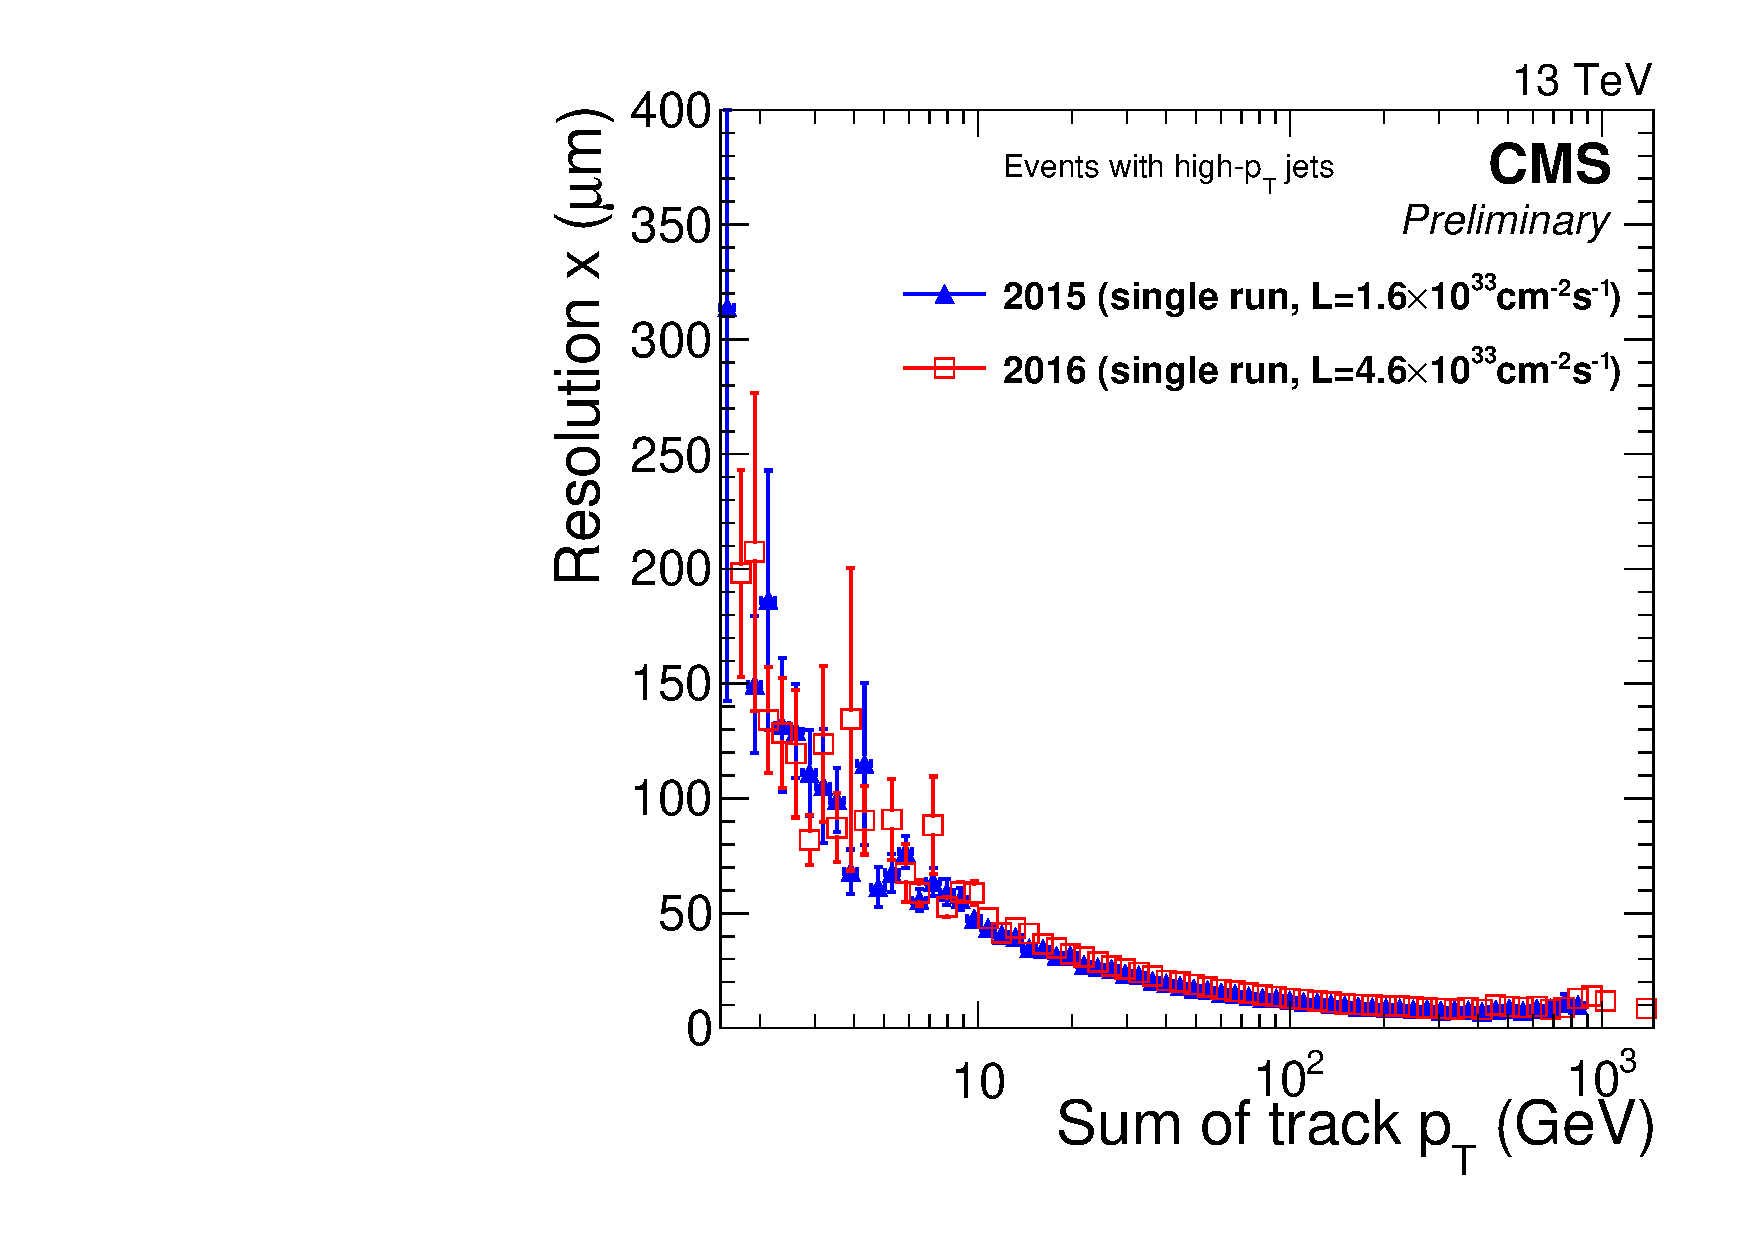
\includegraphics[width=\textwidth]{Figures/Chapter4/resolution_sumpt_x.pdf}
        \caption{}
    \end{subfigure}
    \begin{subfigure}[b]{0.49\textwidth}
        \centering
        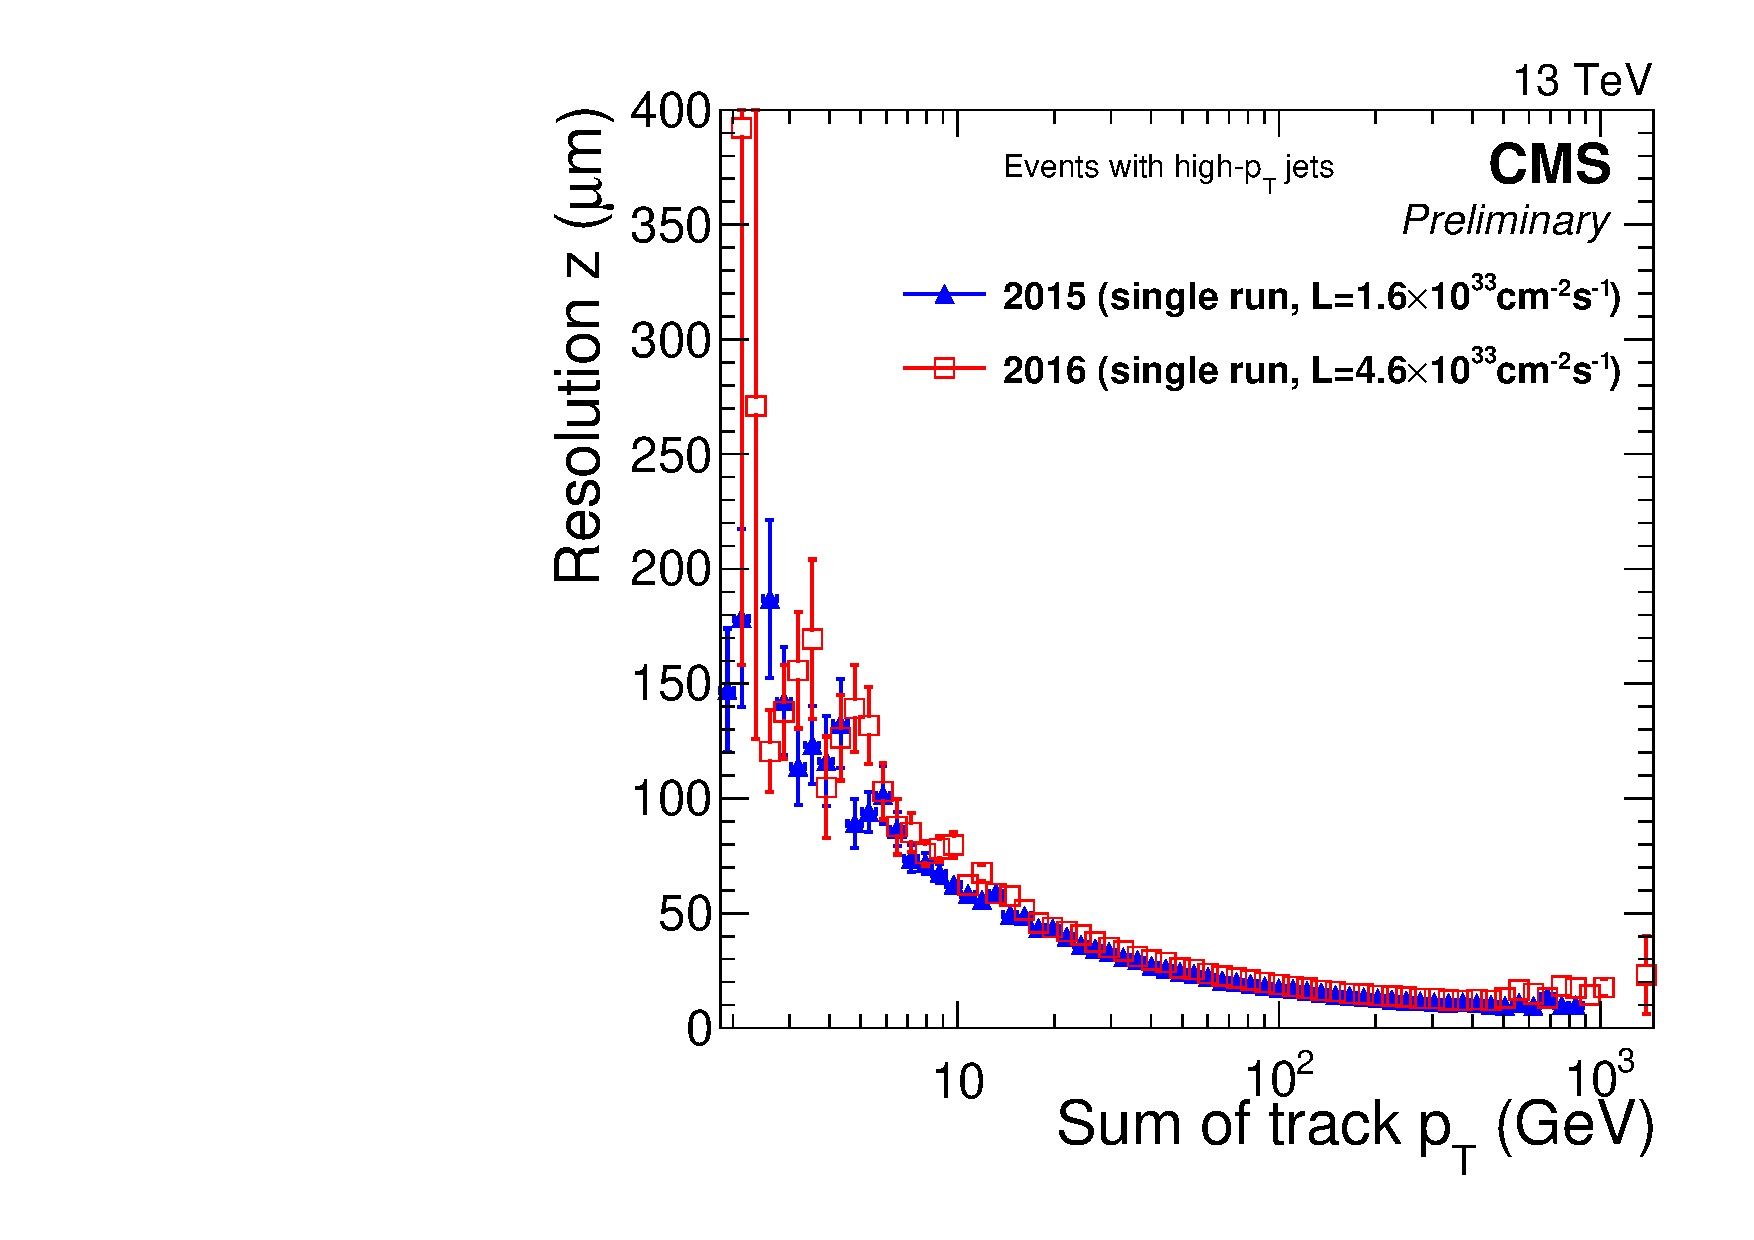
\includegraphics[width=\textwidth]{Figures/Chapter4/resolution_sumpt_z.pdf}
        \caption{}
    \end{subfigure}
\caption[Resolution of the reconstructed transverse and longitudinal positions of the primary vertex using CMS collision data (2015 \& 2016)]{Resolution of the reconstructed PV position in the \textbf{(a)} transverse ($x$) and \textbf{(b)} longitudinal ($z$) directions as a function of the $\sum p_\mathrm{T}$ of the associated tracks. Measurements are shown for pp collisions recorded in 2015 (blue) and 2016 (red). Figures taken from Ref.~\cite{PrimaryVertex_Resolution}.}

\label{Figure:Chapter4_PrimaryVertex_Resolution}
\end{figure}

\subsection{Electron tracking}
\label{Section:Chapter4_ElectronTracking}
Electron reconstruction in CMS leverages both tracking information from the silicon tracker and energy deposits in the ECAL. Two complementary seeding strategies are employed: one utilising energetic ECAL clusters ($E_\mathrm{T} > 4\GeV$), referred to as the \textit{ECAL-based approach}, and the other utilising reconstructed tracks, referred to as the \textit{tracker-based approach}.

As electrons traverse the CMS tracker, they emit a sizeable fraction of their energy as bremsstrahlung photons due to the significant material thickness (see Fig.~\ref{Figure:Chapter3_Tracker_MaterialBudget}). The performance of the \textbf{ECAL-based approach} therefore depends on the ability to recover this radiated energy while minimising contamination from nearby particles. These photons are predominantly emitted along the electron’s direction but become laterally displaced in $\phi$ due to the curvature of the track in the magnetic field. To capture this energy, a \textit{supercluster} is constructed by merging multiple ECAL clusters within a narrow $\eta$ window and an extended $\phi$ window around the expected electron trajectory~\cite{ParticleFlow}. However, this method exhibits significant inefficiencies in high-density environments, such as when electrons are embedded in jets, where overlapping energy deposits from nearby particles can bias the supercluster’s energy and position. It also suffers when back-propagating from the supercluster to the interaction point, as the supercluster may be compatible with multiple hits from other charged particles, increasing the risk of misreconstruction. Further inefficiencies arise for low-$p_\mathrm{T}$ electrons, where the radiated energy is spread over a broad $\phi$ range, preventing complete energy recovery within a single supercluster.

To recover electrons missed by the ECAL-based method, the \textbf{tracker-based} approach is employed. This approach leverages the high efficiency of the iterative tracking algorithm, which can reliably reconstruct both non-radiating and radiating electrons. Tracks with $p_\mathrm{T} > 2\GeV$ from iterative tracking are considered as potential electron seeds. When bremsstrahlung emission is minimal, the corresponding track can be well reconstructed, as indicated by a well-behaved $\chi^2$ from the track fit,\footnote{The chi-squared ($\chi^2$) statistic quantifies the agreement between the measured hit positions and the predicted trajectory of the track. A low $\chi^2$ indicates a good-quality fit and, therefore, a well-reconstructed track.} and propagated safely to the ECAL inner surface for matching with the nearest ECAL cluster. However, when bremsstrahlung is more significant, the pattern recognition may still recover the track, but often with degraded fit quality (\ie fewer associated hits or a larger $\chi^2$). To address this, a preselection is applied based on the number of hits and the $\chi^2$ of the initial fit, after which tracks are refitted using a \textbf{\ac{GSF}} algorithm~\cite{GSF_Algorithm}. Unlike the KF used in standard tracking, the GSF is specifically designed to accommodate the sudden and substantial energy losses along the trajectory.

\subsection{Muon tracking}

Muon reconstruction~\cite{ParticleFlow} in CMS combines information from the dedicated muon detection system with precision tracking from the inner tracker. Three complementary reconstruction strategies are employed, leading to different possible definitions for reconstructed muons:

\begin{itemize}
    \item \textbf{Standalone muon}: In the muon system, hits from each DT or CSC are clustered into track segments, which serve as seeds for pattern recognition. These seeds are used to collect compatible hits across all muon subsystems (DT, CSC, RPC) to reconstruct the muon trajectory. This is referred to as a standalone muon track because the reconstruction is performed using only information from the muon system.
    \item \textbf{Global muon}: Standalone muon tracks are matched to tracks in the inner tracker. If there is a compatible match, a combined fit of the hits from the inner tracker and muon system is performed to form a global muon track.
    \item \textbf{Tracker muon}: Inner tracks with sufficient transverse ($> 0.5\GeV$) and total momenta ($>2.5\GeV$) are extrapolated to the muon system and classified as tracker muons if they are spatially compatible with at least one muon segment.
\end{itemize}

\textit{Global muon reconstruction} is most efficient for muons that traverse multiple muon detector planes. However, at low momenta ($<10\GeV$), larger multiple scattering in the steel return yoke reduces the efficiency of global muon reconstruction, as it becomes more difficult to associate segments in multiple muon stations. In such cases, \textit{tracker muon reconstruction} is more efficient, as it requires only a single matched segment~\cite{CMS_Muon_System_Performance_2}. The high efficiency of both the inner tracker and muon segment reconstruction ensures that approximately 99\% of muons within the detector's acceptance are reconstructed as either global or tracker muons, and often as both.  In such cases, global and tracker muons sharing the same inner track are merged into a single muon candidate.

\subsection{Calorimeter clusters}

The reconstruction of calorimeter-based PF elements in CMS is designed to~\cite{ParticleFlow}:

\begin{itemize}
    \item Identify and measure the energy and direction of stable neutral particles
    \item Distinguish neutral particle energy deposits from those of charged hadrons
    \item Reconstruct electrons along with their associated bremsstrahlung photon energy deposits
    \item Aid the energy measurement of charged hadrons in cases where the track information is imprecise
\end{itemize}

A dedicated clustering algorithm~\cite{ParticleFlow} is applied separately in each calorimeter subsystem, including the barrel and endcap regions of the ECAL and HCAL, as well as the ECAL preshower. For the HF subdetector, clustering is not performed; instead, each cell directly forms an electromagnetic or hadronic cluster. 

\textit{Cluster seeds} are identified in the first step of the algorithm. These are calorimeter cells with energy above a specified threshold that also represent local maxima with respect to their neighbouring cells. In the second step, \textit{topological clusters} are grown from the seeds by adding neighbouring cells that share at least a corner with an existing cluster cell and have energy above a threshold, typically set to twice the noise level. In the final step, an expectation-maximisation algorithm based on a Gaussian mixture model is applied to decompose each topological cluster into one or more individual \textit{``PF'' clusters}.

\section{Particle Flow}
The tracking information and calorimeter clusters described in Section~\ref{Section:Chapter4_Reconstruction_of_PF_elements} form the foundational inputs to the \textit{PF algorithm}. As a single particle generally produces multiple PF elements across the various CMS subdetectors, the reconstruction process begins with a \textit{link algorithm} that connects these elements. The primary limitation of the PF algorithm lies in its dependence on accurately linking detector elements that originate from the same particle. As such, its performance is sensitive to the granularity of the subdetectors, the local density of particles in the event, and the amount of material a particle traverses before reaching the calorimeters and the muon system.

The \textit{linking procedure} begins by evaluating nearby pairs of elements in the $\eta$–$\phi$ plane and, where applicable, defines a distance parameter to quantify the quality of the link. Links between tracks in the central tracker and calorimeter clusters are established by extrapolating a track from its last measured hit in the tracker to different depths in the ECAL (at the expected electron shower maximum) and HCAL (at a depth of one interaction length). A link is created if the extrapolated position falls within the boundaries of the cluster. Similarly, a track-cluster distance parameter is defined as the distance between the extrapolated track position and the cluster position in $\eta$–$\phi$ plane. When multiple HCAL clusters are linked to the same track, or several tracks are associated with the same ECAL cluster, this distance parameter is used to resolve ambiguities by retaining only the link with the smallest value. To recover energy lost via electron bremsstrahlung, tangents to the GSF tracks are extrapolated to the ECAL and used to link clusters within a narrow $\eta$ window ($\Delta\eta < 0.05$), while converted photons are recovered by linking track pairs using a dedicated conversion finder~\cite{DedicatedConversionFinder}. In addition, links between calorimeter clusters (HCAL-ECAL \& ECAL-PS) are established based on their positions in the more granular calorimeter. Similarly, a cluster-cluster distance parameter is defined as the distance between the cluster positions in the $\eta-\phi$ plane. As in the case of track–cluster associations, when multiple clusters are compatible, only the link with the smallest distance is retained. Finally, links between tracks in the central tracker and information in the muon system are established through a global fit, with the distance parameter defined as the $\chi^2$ of the fit. In cases where multiple associations are possible, only the link with the lowest $\chi^2$ is retained to ensure the most compatible match.

Once all valid links are established, groups of interconnected elements, either through direct or indirect links, are assembled into \textit{PF blocks}. Each PF block is processed by the PF algorithm, which operates on the block following a well-defined sequence of steps to reconstruct and identify a set of particles. The procedure is as follows:

\begin{enumerate}
    \item \textbf{PF muons}: Global muons present within the block are identified as PF muons if their associated track is consistent with minimal energy deposition in the calorimeters. Once identified, the corresponding tracker and muon elements are removed from the block.
    \item \textbf{PF electrons}: Tracks not previously identified as muons are submitted to a pre-identification step that selects candidate electrons based on characteristic bremsstrahlung patterns observed in the tracker. As described in Section~\ref{Section:Chapter4_ElectronTracking}, these candidates are refitted with a Gaussian Sum Filter (GSF), and a multivariate discriminant combining tracking and ECAL variables is applied. If the candidate passes the discriminant, it is identified as a PF electron, and the associated track and ECAL clusters are removed from the block.
    \item \textbf{PF photons \& PF neutral hadrons}: Non-compatible calorimeter clusters with track momentum are interpreted as neutral particles, following:
    \begin{itemize}
        \item Depending on the relative energy in each calorimeter, both a PF photon (from ECAL) and a PF neutral hadron (from HCAL) may be created to account for the excess.
        \item If the excess energy is primarily in the ECAL and exhibits electromagnetic shower characteristics, only a PF photon is created.
        \item ECAL and HCAL clusters with no associated tracks are interpreted as PF photons and PF neutral hadrons, respectively
    \end{itemize}
\end{enumerate}

\section{Object identification}
\label{Section:Chapter4_Object_Identification}

The final output of the PF algorithm is a list of reconstructed particles, referred to as \textit{PF candidates}. However, PF does not inherently guarantee that the candidates correspond to genuine prompt physics objects. Therefore, dedicated identification (ID) algorithms are required to translate these PF candidates into physics objects suitable for analysis. This section serves to describe the object identification strategies used in this thesis.

\subsection{Electrons}

Electrons are identified using a \ac{MVA} approach, where a \ac{BDT} algorithm is employed to distinguish genuine prompt electrons from backgrounds. These backgrounds include electrons from photon conversions, misidentified hadrons, and non-prompt electrons from the decay of hadrons. The set of discriminating variables used by the BDT can be grouped into the following categories:

\begin{itemize}
    \item \textbf{Track-cluster matching observables}: These variables compare measurements obtained from the ECAL and the tracker, including both geometrical matching between the ECAL supercluster and the tracker, as well as energy-momentum matching.
    \item \textbf{Calorimetric observables}: These variables are purely calorimetric and are used to improve the separation between genuine and misidentified electrons. One example is the transverse shape of EM showers in the ECAL, where the typically narrow profile of EM showers is exploited in contrast to the broader shape of hadronic showers. Additional calorimetric observables include the hadronic-to-electromagnetic energy ratio ($H/E$), which is expected to be small for electrons, and the energy deposited in the HCAL and preshower (in the endcaps), which further helps to discriminate against hadronic backgrounds.
    \item \textbf{Tracking observables}: These variables are used to enhance discrimination between electrons and charged hadrons by leveraging detailed information from the GSF track fit, as well as discrepancies between the GSF and KF track reconstructions.
\end{itemize}

A working point corresponding to 90\% signal efficiency is used in this thesis, meaning that approximately 90\% of genuine prompt electrons are correctly identified~\cite{ElectronID_Performance}. To accommodate different analysis needs, two versions of the BDT discriminator are employed: one that includes isolation variables during training, and one that does not, allowing flexibility in environments with varying levels of surrounding activity. 

In addition to the BDT-based electron identification, isolation requirements are essential for further suppressing backgrounds from misidentified jets or genuine electrons within jets arising from heavy-flavour decays. These background electrons are typically accompanied by significant nearby energy deposits, which can be effectively rejected by imposing an isolation criterion. A simple isolation variable is based on detector-based isolation. This approach computes the scalar sum of transverse energy deposits in the ECAL or HCAL, or the scalar sum of the $p_\mathrm{T}$ of tracks originating from the primary collision vertex, within a cone of radius $\Delta R$ (typically 0.3 or 0.4) around the electron direction. 

A more refined isolation variable is the \textit{PF isolation} ($I_{\text{PF}}^e$, which utilises PF candidates reconstructed within a cone around the electron's direction:

\begin{equation_pad}
    I_{\text{PF}}^e = \frac{1}{p_\mathrm{T}^e} \left( \sum_{\text{h}^{\pm}} p_\mathrm{T} + \text{max} \left[0, \sum_{\text{h}^{0}} p_\mathrm{T} + \sum_{\gamma} p_\mathrm{T} - \rho A_{\text{eff}}\right]  \right)
\end{equation_pad}

where the sums include all PF charged hadrons ($h^\pm$) originating from the primary vertex, neutral hadrons ($h^0$), and photons ($\gamma$). The term $\rho A_{\text{eff}}$ accounts for the contribution from PU interactions.





% \subsection{Muons}



% \subsection{Jets}

% \subsection{Missing transverse energy}

% \subsection{Taus}